%package list
\documentclass{article}
\usepackage[top=3cm, bottom=3cm, outer=3cm, inner=3cm]{geometry}
\usepackage{multicol}
\usepackage{graphicx}
\usepackage{url}
%\usepackage{cite}
\usepackage{hyperref}
\usepackage{array}
%\usepackage{multicol}
\newcolumntype{x}[1]{>{\centering\arraybackslash\hspace{0pt}}p{#1}}
\usepackage{natbib}
\usepackage{pdfpages}
\usepackage{multirow}
\usepackage[normalem]{ulem}
\useunder{\uline}{\ul}{}
\usepackage{svg}
\usepackage{xcolor}
\usepackage{listings}
\lstdefinestyle{ascii-tree}{
    literate={├}{|}1 {─}{--}1 {└}{+}1 
  }
\lstset{basicstyle=\ttfamily,
  showstringspaces=false,
  commentstyle=\color{red},
  keywordstyle=\color{blue}
}
%\usepackage{booktabs}
\usepackage{caption}
\usepackage{subcaption}
\usepackage{float}
\usepackage{array}

\newcolumntype{M}[1]{>{\centering\arraybackslash}m{#1}}
\newcolumntype{N}{@{}m{0pt}@{}}


%%%%%%%%%%%%%%%%%%%%%%%%%%%%%%%%%%%%%%%%%%%%%%%%%%%%%%%%%%%%%%%%%%%%%%%%%%%%
%%%%%%%%%%%%%%%%%%%%%%%%%%%%%%%%%%%%%%%%%%%%%%%%%%%%%%%%%%%%%%%%%%%%%%%%%%%%
\newcommand{\itemEmail}{mvelasquea@unsa.edu.pe}
\newcommand{\itemStudent}{Mikhail Gabino Velasque Arcos}
\newcommand{\itemCourse}{ FUNDAMENTOS DE LA PROGRAMACION II}
\newcommand{\itemCourseCode}{20214260}
\newcommand{\itemSemester}{II}
\newcommand{\itemUniversity}{Universidad Nacional de San Agustín de Arequipa}
\newcommand{\itemFaculty}{Facultad de Ingeniería de Producción y Servicios}
\newcommand{\itemDepartment}{Departamento Académico de Ingeniería de Sistemas e Informática}
\newcommand{\itemSchool}{Escuela Profesional de Ingeniería de Sistemas}
\newcommand{\itemAcademic}{2023 - B}
\newcommand{\itemInput}{Del 15 de Enero del 2024}
\newcommand{\itemOutput}{Al 02 de Febrero del 2024}
\newcommand{\itemPracticeNumber}{23}
\newcommand{\itemTheme}{Proyecto final del laboratorio fp2}
%%%%%%%%%%%%%%%%%%%%%%%%%%%%%%%%%%%%%%%%%%%%%%%%%%%%%%%%%%%%%%%%%%%%%%%%%%%%
%%%%%%%%%%%%%%%%%%%%%%%%%%%%%%%%%%%%%%%%%%%%%%%%%%%%%%%%%%%%%%%%%%%%%%%%%%%%

\usepackage[english,spanish]{babel}
\usepackage[utf8]{inputenc}
\AtBeginDocument{\selectlanguage{spanish}}
\renewcommand{\figurename}{Figura}
\renewcommand{\refname}{Referencias}
\renewcommand{\tablename}{Tabla} %esto no funciona cuando se usa babel
\AtBeginDocument{%
	\renewcommand\tablename{Tabla}
}

\usepackage{fancyhdr}
\pagestyle{fancy}
\fancyhf{}
\setlength{\headheight}{30pt}
\renewcommand{\headrulewidth}{1pt}
\renewcommand{\footrulewidth}{1pt}
\fancyhead[L]{\raisebox{-0.2\height}{
\includegraphics[width=3cm]{img/logo_episunsa.png}}}
\fancyhead[C]{\fontsize{7}{7}\selectfont	\itemUniversity \\ \itemFaculty \\ \itemDepartment \\ \itemSchool \\ \textbf{\itemCourse}}
\fancyhead[R]{\raisebox{-0.2\height}{
\includegraphics[width=1.2cm]{img/logo_abet}}}
\fancyfoot[L]{Estudiante Mikhail Gabino Velasque Arcos}
\fancyfoot[C]{\itemCourse}
\fancyfoot[R]{Página \thepage}

% para el codigo fuente
\usepackage{listings}
\usepackage{color, colortbl}
\definecolor{dkgreen}{rgb}{0,0.6,0}
\definecolor{gray}{rgb}{0.5,0.5,0.5}
\definecolor{mauve}{rgb}{0.58,0,0.82}
\definecolor{codebackground}{rgb}{0.95, 0.95, 0.92}
\definecolor{tablebackground}{rgb}{0.8, 0, 0}

\lstset{frame=tb,
	language=bash,
	aboveskip=3mm,
	belowskip=3mm,
	showstringspaces=false,
	columns=flexible,
	basicstyle={\small\ttfamily},
	numbers=none,
	numberstyle=\tiny\color{gray},
	keywordstyle=\color{blue},
	commentstyle=\color{dkgreen},
	stringstyle=\color{mauve},
	breaklines=true,
	breakatwhitespace=true,
	tabsize=3,
	backgroundcolor= \color{codebackground},
}

\begin{document}
	
	\vspace*{10px}
	
	\begin{center}	
		\fontsize{17}{17} \textbf{ Proyecto final}
	\end{center}
	\centerline{\textbf{\Large Tema: ----}}
	%\vspace*{0.5cm}	

	\begin{flushright}
		\begin{tabular}{|M{2.5cm}|N|}
			\hline 
			\rowcolor{tablebackground}
			\color{white} \textbf{Nota}  \\
			\hline 
			     \\[30pt]
			\hline 			
		\end{tabular}
	\end{flushright}	

	\begin{table}[H]
		\begin{tabular}{|x{4.7cm}|x{4.8cm}|x{4.8cm}|}
			\hline 
			\rowcolor{tablebackground}
			\color{white} \textbf{Estudiante} & \color{white}\textbf{Escuela}  & \color{white}\textbf{Asignatura}   \\
			\hline 
			{\itemStudent \par \itemEmail} & \itemSchool & {\itemCourse \par Semestre: \itemSemester \par Código: \itemCourseCode}     \\
			\hline 			
		\end{tabular}
	\end{table}		
	
	\begin{table}[H]
		\begin{tabular}{|x{4.7cm}|x{4.8cm}|x{4.8cm}|}
			\hline 
			\rowcolor{tablebackground}
			\color{white}\textbf{Laboratorio} & \color{white}\textbf{Tema}  & \color{white}\textbf{Duración}   \\
			\hline 
			\itemPracticeNumber & \itemTheme & 04 horas   \\
			\hline 
		\end{tabular}
	\end{table}
	
	\begin{table}[H]
		\begin{tabular}{|x{4.7cm}|x{4.8cm}|x{4.8cm}|}
			\hline 
			\rowcolor{tablebackground}
			\color{white}\textbf{Semestre académico} & \color{white}\textbf{Fecha de inicio}  & \color{white}\textbf{Fecha de entrega}   \\
			\hline 
			\itemAcademic & \itemInput &  \itemOutput  \\
			\hline 
		\end{tabular}
	\end{table}
%%%%%%%%%%%%%%%%%%%%%%%%%%%%%%%%%%%%%%%%%%%%%%%%%%%%%%%%%%%%%%%%%%%%%%%%%%%%
%%%%%%%%%%%%%%%%%%%%%%%%%%%%%%%%%%%%%%%%%%%%%%%%%%%%%%%%%%%%%%%%%%%%%%%%%%%%
	\section{Actividad}
	\begin{itemize}		
		\item Realizar el videojuego final en base a todo lo avanzado durante el laboratio de Fundamentos de la Progamacion II
		
		\end{itemize}
	\section{Equipos, materiales y temas utilizados}
	\begin{itemize}
		\item Git , Git hub , clases, Diagramas UML ,herencia , herencia multiple
		\item VIM 9.0.
		\item OpenJDK 64-Bits 17.0.7.
		\item Git 2.39.2.
		\item Cuenta en GitHub con el correo institucional.
		\item Programación Orientada a Objetos.
		\item Jframe
	\end{itemize}
	
	\section{URL de Repositorio Github}
	\begin{itemize}
		\item URL del Repositorio GitHub para clonar o recuperar.
			\item URL :https://github.com/mvelasquea/fp2-23b.git
\end{itemize}
	\section{Equipos, materiales y temas utilizados}
	\begin{itemize}
		\item Git , Git hub , clases, Diagramas UML ,herencia , herencia multiple
		\item VIM 9.0.
		\item OpenJDK 64-Bits 17.0.7.
		\item Git 2.39.2.
		\item Cuenta en GitHub con el correo institucional.
		\item Programación Orientada a Objetos.
	\end{itemize}
	
	\section{URL de Repositorio Github}
	\begin{itemize}
		\item URL del Repositorio GitHub para clonar o recuperar.
			\item URL :https://github.com/mvelasquea/fp2-23b.git

	\end{itemize}
	
	\section{Ejercicio 1:Videojuego final(Jframe)}
	
	\subsection{la clase main}
		
	\begin{lstlisting}[language=bash,caption={CLASE MAIN o "ViDEOJUEGO"}][H]
	

import javax.swing.*;
import java.awt.event.ActionEvent;
import java.awt.event.ActionListener;

public class Videojuego {
    public static void main(String[] args) {
        int option;

        do {
            // Muestra la ventana del menú
            MenuFrame menuFrame = new MenuFrame();

            Mapa terreno = new Mapa();
            Tablero tabla = new Tablero(terreno.getEjercito1(), terreno.getEjercito2());
            terreno.imprimirDatosFinales();
            juego(terreno, tabla);

            option = JOptionPane.showConfirmDialog(null, "¿Desea salir?", "Salir", JOptionPane.YES_NO_OPTION);

        
            menuFrame.dispose();

        

        } while (option == JOptionPane.NO_OPTION);

        System.exit(0);
    }

    public static void juego(Mapa terreno, Tablero tabla) {
        Ejercito e1 = terreno.getEjercito1();
        Ejercito e2 = terreno.getEjercito2();
        int turno = 0;
        JOptionPane.showMessageDialog(null, "Bienvenido al simulador");
        tabla.repintarTablero();
        do {
            if (turno % 2 == 0) {
                int x = 0, y = 0, tox = 0, toy = 0;
                do {
                    JOptionPane.showMessageDialog(null, "Turno del reino Azul");
                    int arr[] = tabla.getCoordenadas();
                    x = arr[0];
                    y = arr[1];
                    int toarr[] = tabla.getCoordenadas();
                    tox = toarr[0];
                    toy = toarr[1];
                    x--;
                    y--;
                    tox--;
                    toy--;
                } while (Ejercito.validar(e1, e2, x, y, tox, toy));
                Ejercito.mover(e1, e2, x, y, tox, toy);
            } else {
                int x = 0, y = 0, tox = 0, toy = 0;
                do {
                    JOptionPane.showMessageDialog(null, "Turno del reino Rojo");
                    int arr[] = tabla.getCoordenadas();
                    x = arr[0];
                    y = arr[1];
                    int toarr[] = tabla.getCoordenadas();
                    tox = toarr[0];
                    toy = toarr[1];
                    x--;
                    y--;
                    tox--;
                    toy--;
                } while (Ejercito.validar(e2, e1, x, y, tox, toy));
                Ejercito.mover(e2, e1, x, y, tox, toy);
            }
            tabla.repintarTablero();
            turno++;
        } while (Ejercito.winner(e1, e2));
    }

    public static class MenuFrame extends JFrame {
        public MenuFrame() {
            setTitle("Menú del Juego");
            setSize(400, 200);
            setDefaultCloseOperation(JFrame.DISPOSE_ON_CLOSE);
            setLayout(new BoxLayout(getContentPane(), BoxLayout.Y_AXIS));  // Usar BoxLayout en eje Y

            // Agrega aquí los elementos del menú (botones, opciones, etc.)

            // Botón Partida Rápida
            JButton botonPartidaRapida = new JButton("Partida Rápida");
            botonPartidaRapida.addActionListener(e -> {
                Mapa terreno = new Mapa();
                Tablero tabla = new Tablero(terreno.getEjercito1(), terreno.getEjercito2());
                terreno.imprimirDatosFinales();
                juego(terreno, tabla);
            });
            add(botonPartidaRapida);

            // Botón Partida Personalizada
            JButton botonPartidaPersonalizada = new JButton("Partida Personalizada");
            botonPartidaPersonalizada.addActionListener(e -> {
                Mapa terreno = new Mapa();
              
                Tablero tabla = new Tablero(terreno.getEjercito1(), terreno.getEjercito2());
                terreno.imprimirDatosFinales();
                juego(terreno, tabla);
            });
            add(botonPartidaPersonalizada);

            // Botón Salir
            JButton botonSalir = new JButton("Salir");
            botonSalir.addActionListener(e -> {
                int confirm = JOptionPane.showOptionDialog(
                        null,
                        "¿Desea salir del juego?",
                        "Salir",
                        JOptionPane.YES_NO_OPTION,
                        JOptionPane.QUESTION_MESSAGE,
                        null, null, null);

                if (confirm == JOptionPane.YES_OPTION) {
                    System.exit(0);
                }
            });
            add(botonSalir);

            setLocationRelativeTo(null);
            setVisible(true);
        }
    }
}

}
	\end{lstlisting}	
	
	
	\subsection{Creando la clase Tablero}
		
	\begin{lstlisting}[language=bash,caption={CLASE Tablero}][H]
	



import javax.swing.*;
import javax.swing.border.Border;
import java.awt.*;
import java.awt.event.ActionEvent;
import java.awt.event.ActionListener;
import java.io.FileWriter;
import java.io.IOException;
import java.io.PrintWriter;
import java.util.concurrent.CountDownLatch;

public class Tablero extends JFrame {
    private static final int ANCHO = 800;
    private static final int ALTO = 1000;
    private static final int FILAS = 10;
    private static final int COLUMNAS = 10;

    private Ejercito e1;
    private Ejercito e2;
    

private synchronized void createMenu() {
    JMenuBar menuBar = new JMenuBar();
    setJMenuBar(menuBar);

    JMenu menuPartida = new JMenu("Partida");
    menuBar.add(menuPartida);

    JMenuItem partidaRapida = new JMenuItem("Partida Rápida");
    JMenuItem partidaPersonalizada = new JMenuItem("Partida Personalizada");
    JMenuItem salir = new JMenuItem("Salir");

    menuPartida.add(partidaRapida);
    menuPartida.add(partidaPersonalizada);
    menuPartida.addSeparator();
    menuPartida.add(salir);

    partidaRapida.addActionListener(new ActionListener() {
        @Override
        public void actionPerformed(ActionEvent e) {
            // Lógica para partida rápida
            // Puedes llamar a métodos adicionales o ajustar el estado del juego
        }
    });
    partidaPersonalizada.addActionListener(new ActionListener() {
        @Override
        public void actionPerformed(ActionEvent e) {
            // Lógica para partida personalizada
            // Puedes abrir un nuevo cuadro de diálogo para configurar opciones
        }
    });

    salir.addActionListener(new ActionListener() {
        @Override
        public void actionPerformed(ActionEvent e) {
            // Lógica para salir
            int confirm = JOptionPane.showOptionDialog(
                    null,
                    "¿Desea salir del juego?",
                    "Salir",
                    JOptionPane.YES_NO_OPTION,
                    JOptionPane.QUESTION_MESSAGE,
                    null, null, null);

            if (confirm == JOptionPane.YES_OPTION) {
                System.exit(0);
            }
        }
    });
}


    public Tablero(Ejercito e1, Ejercito e2) {
        setTitle("Campo de batalla");
        setSize(ANCHO, ALTO);
        setLayout(new GridLayout(FILAS + 2, COLUMNAS + 1, 2, 2));
        this.e1 = e1;
        this.e2 = e2;
        createContents();
        setDefaultCloseOperation(EXIT_ON_CLOSE);
        setVisible(true);
    }

    public synchronized void createContents() {

        JLabel[] columnas = new JLabel[COLUMNAS];
        char[] cols = {'A', 'B', 'C', 'D', 'E', 'F', 'G', 'H', 'I', 'J'};
        for (int i = 0; i < COLUMNAS; i++) {
            columnas[i] = new JLabel(cols[i] + "");
            columnas[i].setHorizontalAlignment(JLabel.CENTER);
            columnas[i].setVerticalAlignment(JLabel.CENTER);
            Border border = BorderFactory.createLineBorder(Color.GREEN, 2);

            columnas[i].setFont(new Font("Arial", Font.BOLD, 30));
            columnas[i].setBorder(border);
            add(columnas[i]);
        }

        JLabel[] filas = new JLabel[FILAS];
        for (int i = 0; i < FILAS; i++) {
            filas[i] = new JLabel((i + 1) + "");
            filas[i].setVerticalAlignment(JLabel.CENTER);
            filas[i].setHorizontalAlignment(JLabel.CENTER);
            filas[i].setFont(new Font("Arial", Font.BOLD, 30));
            Border border = BorderFactory.createLineBorder(Color.GREEN, 2);
            filas[i].setBorder(border);
            add(filas[i]);
        }
        for (int i = 0; i < COLUMNAS + 1; i++) {
            if (i == 0) {
                add(new JLabel());
            } else {
                add(columnas[i - 1]);
            }
        }

        for (int i = 0; i < FILAS; i++) {
            add(filas[i]);
            for (int j = 0; j < COLUMNAS; j++) {
                JButton boton = new JButton("");
                for (Soldado s : e1.getSoldados()) {
                    if (s.getFila() == i && s.getColumna() == j) {
                        boton = new JButton(s.impresionTabla());
                        boton.setBackground(Color.blue);
                        break;
                    }
                }
                for (Soldado s : e2.getSoldados()) {
                    if (s.getFila() == i && s.getColumna() == j) {
                        boton = new JButton(s.impresionTabla());
                        boton.setBackground(Color.red);
                        break;
                    }
                }
                boton.addActionListener(new ButtonListener(i, j));
                add(boton);
            }
        }
    }
    private void ajustarEstiloBoton(JButton boton) {
        boton.setFont(new Font("Arial", Font.BOLD, 18));  // Cambia la fuente y el tamaño
        boton.setForeground(Color.WHITE);  // Cambia el color del texto
    
    }
    private int fila = -1;
    private int columna = -1;
    private CountDownLatch latch = new CountDownLatch(1);

    private class ButtonListener implements ActionListener {
        private int f;
        private int c;
        public ButtonListener(int f, int c) {
            this.f = f;
            this.c = c;
        }
        public void actionPerformed(ActionEvent e) {
            fila = f;
            columna = c;
            latch.countDown(); 
        }
    }
    public int[] getCoordenadas() {
        try {
            latch.await(); 
        } catch (InterruptedException e) {
            e.printStackTrace();
        }
        int[] arr = new int[2];
        arr[0] = fila + 1;
        arr[1] = columna + 1;
        fila = -1;
        columna = -1;
        latch = new CountDownLatch(1);
        return arr;
    }

    public void repintarTablero() {
        getContentPane().removeAll(); 
        createContents(); 
        revalidate(); 
        repaint();
    }
}
	\end{lstlisting}		
	
	
	
	\begin{lstlisting}[language=bash,caption={CLASE Mapa}][H]
	

import java.util.HashMap;
import java.util.Random;

public class Mapa {
    private Ejercito e1 = new Ejercito();
    private Ejercito e2 = new Ejercito();
    private int tipoMapa;
    private HashMap<Integer, String> terr = new HashMap<Integer, String>() {{
        put(1, "Bosque");
        put(2, "Campo Abierto");
        put(3, "Montañas");
        put(4, "Desierto");
        put(5, "Playa");
    }};
    private HashMap<Integer, String> reinos = new HashMap<Integer, String>() {{
        put(1, "Inglaterra");
        put(2, "Francia");
        put(3, "Castilla-Aragon");
        put(4, "Moros");
        put(5, "Sacro Imperio Romano-Germanico");
    }};
    private boolean[][] posiciones = new boolean[10][10];
    private int numeroEjercito1;

    public Mapa() {
        Random random = new Random();
        int numero1 = random.nextInt(5) + 1;
        int numero2;
        do {
            numero2 = random.nextInt(5) + 1;
        } while (numero2 == numero1);
        e1.setReino(numero1);
        e2.setReino(numero2);

        tipoMapa = (int) (Math.random() * 5 + 1);
        generarEjercito(e1, 1);
        generarEjercito(e2, 2);
    }

    private void generarEjercito(Ejercito e, int num) {
        int numEspada = 0;
        int numArque = 0;
        int numCaball = 0;
        int numLanc = 0;
        do {
            numEspada = (int) (Math.random() * 9 + 1);
            numArque = (int) (Math.random() * 9 + 1);
            numCaball = (int) (Math.random() * 9 + 1);
            numLanc = (int) (Math.random() * 9 + 1);

        } while ((numEspada + numArque + numCaball + numLanc) > 10);
        int numEjercito = numEspada + numArque + numCaball + numLanc;
        this.numeroEjercito1 = numEjercito;
        genSoldados(e, numEspada, numArque, numCaball, numLanc, 2);
        aumentarVida();

    }

    private void genSoldados(Ejercito e, int n1, int n2, int n3, int n4, int ejer) {
        boolean isEsp = true;
        for (int i = 0; i < n1; i++) {
            String nombre = "Espadachin" + i + "x" + ejer;
            int fila = 0;
            int columna = 0;
            do {
                fila = (int) (Math.random() * 9);
                columna = (int) (Math.random() * 9);
            } while (posiciones[fila][columna]);
            posiciones[fila][columna] = true;
            Espadachin s = null;
            if (e.getReino() == 1 && isEsp) {
                nombre = "EspadachinReal" + i + "x" + ejer;
                s = new EspadachinReal(nombre, fila, columna, 1);
                isEsp = false;
            } else if (e.getReino() == 3 && isEsp) {
                nombre = "EspadachinConquistador" + i + "x" + ejer;
                s = new EspadachinConquistador(nombre, fila, columna, 3);
                isEsp = false;
            } else if (e.getReino() == 5 && isEsp) {
                nombre = "EspadachinTeutonico" + i + "x" + ejer;
                s = new EspadachinTeutonico(nombre, fila, columna, 5);
                isEsp = false;
            } else {
                s = new Espadachin(nombre, fila, columna, e.getReino());
            }
            e.getSoldados().add(s);
        }
        for (int i = 0; i < n2; i++) {
            String nombre = "Arquero" + i + "x" + ejer;
            int fila = 0;
            int columna = 0;
            do {
                fila = (int) (Math.random() * 9);
                columna = (int) (Math.random() * 9);
            } while (posiciones[fila][columna]);
            posiciones[fila][columna] = true;
            Arquero s = new Arquero(nombre, fila, columna, e.getReino());
            e.getSoldados().add(s);
        }
        boolean isC = true;
        for (int i = 0; i < n3; i++) {
            String nombre = "Caballero" + i + "x" + ejer;
            int fila = 0;
            int columna = 0;
            do {
                fila = (int) (Math.random() * 9);
                columna = (int) (Math.random() * 9);
            } while (posiciones[fila][columna]);
            posiciones[fila][columna] = true;
            Caballero s = null;
            if (e.getReino() == 2 && isC) {
                nombre = "CaballeroFranco" + i + "x" + ejer;
                s = new CaballeroFranco(nombre, fila, columna, 2);
                isC = false;
            } else if (e.getReino() == 4 && isC) {
                nombre = "CaballeroMoro" + i + "x" + ejer;
                s = new CaballeroMoro(nombre, fila, columna, 4);
                isC = false;
            } else {
                s = new Caballero(nombre, fila, columna, e.getReino());
            }
            e.getSoldados().add(s);
        }
        for (int i = 0; i < n4; i++) {
            String nombre = "Lancero" + i + "x" + ejer;
            int fila = 0;
            int columna = 0;
            do {
                fila = (int) (Math.random() * 9);
                columna = (int) (Math.random() * 9);
            } while (posiciones[fila][columna]);
            posiciones[fila][columna] = true;
            Lancero s = new Lancero(nombre, fila, columna, e.getReino());
            e.getSoldados().add(s);
        }
    }

    public Ejercito getEjercito1() {
        return e1;
    }

    public Ejercito getEjercito2() {
        return e2;
    }

    public void aumentarVida() {
        if (e1.getReino() == this.tipoMapa || (e1.getReino() == 5 && this.tipoMapa == 1 || e1.getReino() == 5 && this.tipoMapa == 2)) {
            for (Soldado s : e1.getSoldados()) {
                s.setVidaActual(s.getVidaActual() + 1);
            }
        }
        if (e2.getReino() == this.tipoMapa || (e2.getReino() == 5 && this.tipoMapa == 1 || e2.getReino() == 5 && this.tipoMapa == 2)) {
            for (Soldado s : e2.getSoldados()) {
                s.setVidaActual(s.getVidaActual() + 1);
            }
        }
    }

    public void imprimirDatosFinales() {
        String content = "Ejercito 1: " + reinos.get(e1.getReino()) + "\n" +
                "Cantidad total de soldados creados: " + e1.getSoldados().size() + "\n" +
                "Espadachines: " + e1.getCantidadEsp() + "\n" +
                "Arqueros: " + e1.getCantidadArq() + "\n" +
                "Caballeros: " + e1.getCantidadCab() + "\n" +
                "Lanceros: " + e1.getCantidadLan() + "\n" +
                "\n" +
                "Ejercito 2: " + reinos.get(e2.getReino()) + "\n" +
                "Cantidad total de soldados creados: " + e2.getSoldados().size() + "\n" +
                "Espadachines: " + e2.getCantidadEsp() + "\n" +
                "Arqueros: " + e2.getCantidadArq() + "\n" +
                "Caballeros: " + e2.getCantidadCab() + "\n" +
                "Lanceros: " + e2.getCantidadLan() + "\n";

        String additionalInfo = "El territorio es: " + terr.get(this.tipoMapa) + "\n";

        new InfoFrame("Datos Finales", content, additionalInfo).setLocation(1000, 500);
    }
}

	\end{lstlisting}	
	
	
			
	\begin{lstlisting}[language=bash,caption={CLASE InfoFrame}][H]
	

import javax.swing.*;
import java.awt.*;

public class InfoFrame extends JFrame {
    private JTextArea textArea;

    public InfoFrame(String title, String content, String additionalInfo) {
        setTitle(title);
        setSize(400, 400);
        setDefaultCloseOperation(JFrame.DISPOSE_ON_CLOSE);

        // Crear el área de texto una sola vez
        this.textArea = new JTextArea();
        this.textArea.setEditable(false);
        this.textArea.setFont(new Font("Arial", Font.PLAIN, 16)); // Cambia el tipo de fuente y el tamaño

        JScrollPane scrollPane = new JScrollPane(this.textArea);
        add(scrollPane);

        setLocationRelativeTo(null);
        setVisible(true);

        // Establecer el contenido directamente en el JTextArea
        String styledContent = content + "\n" + additionalInfo;
        this.textArea.setText(styledContent);
    }

    public JTextArea getTextArea() {
        return textArea;
    }
}

	\end{lstlisting}	
	
	
	\subsection{Resultados}
	
	\begin{itemize}	
		\item Se crea un tablero  mostrando cada uno de los soldados consus respectivos colores o bandos
	
	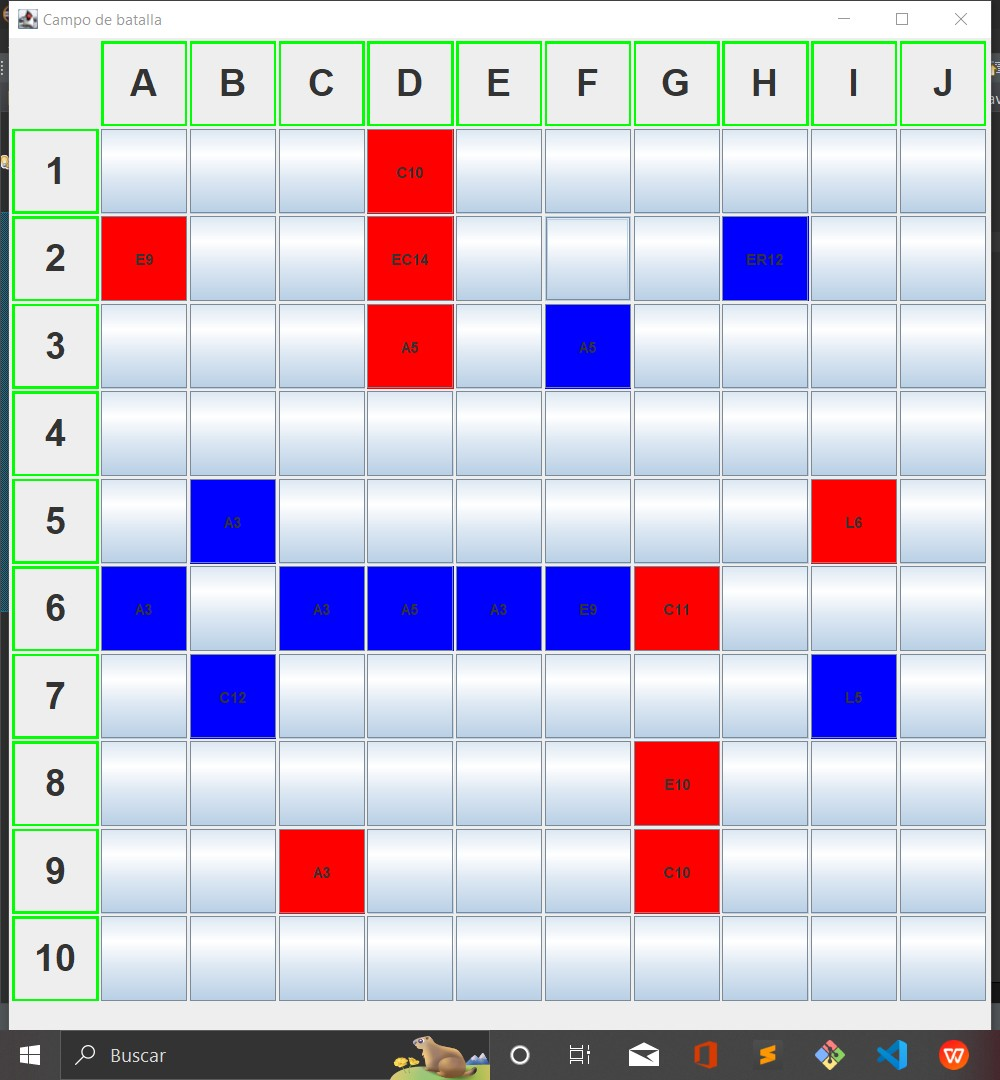
\includegraphics[scale=0.45]{img/captura1.jpeg} 
\item Resultados

	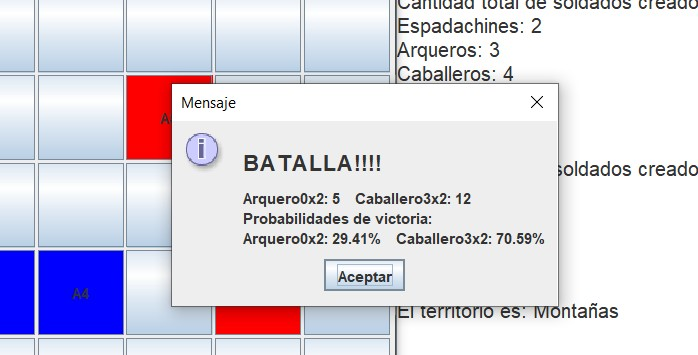
\includegraphics[scale=0.5]{img/captura2.jpeg} 
	
	
\item -
	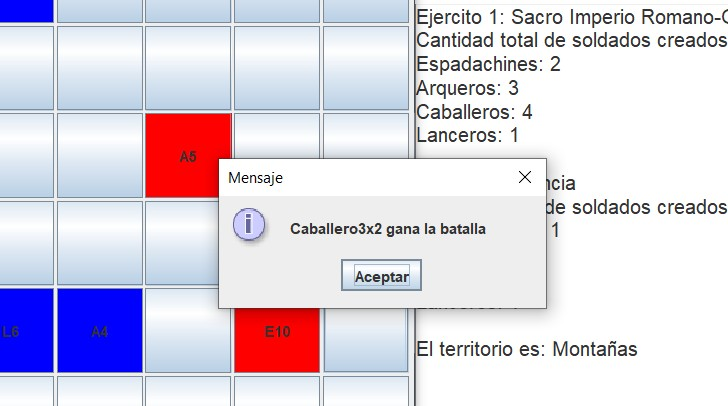
\includegraphics[scale=0.5]{img/captura3.jpeg} 
	\end{itemize}
	
\begin{lstlisting}[style=ascii-tree]
lab20/
|--- Videojuego.java
|--- soldado.java
|--- lancero.java
|--- gitignore.java
|--- Caballero.java
|--- Espadachin.java
|--- Arquero.java
|--- Ejercito.java
|--- Ejercito.java

|--- latex
    |--- img
    |   |--- logo_abet.png
    |   |--- logo_episunsa.png
    |   |--- logo_unsa.jpg
    |   |--- captura1.png    
    |   |--- captura2.png    

    |--- latex_Lab20_COMPLETADO.pdf    
    |--- latex_Lab20_COMPLETADO.tex
    |--- src
        |---Videojuego.java
\end{lstlisting}    













			
\end{document}